
\begin{minipage}{0.49\textwidth}
\caption*{
tip pattern mode
}
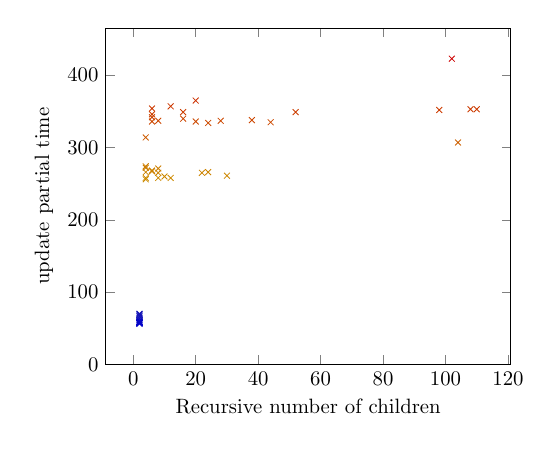
\begin{tikzpicture}[scale=0.75]
\begin{axis}[ymin=0, xlabel={Recursive number of children}, ylabel={update partial time}] \addplot[mark=x, color=blue, scatter, only marks] coordinates {
(2,64) (4,258) (2,57) (8,337) (10,260) (12,258) (2,57) (2,57) (6,336) (2,59) (2,56) (6,346) (8,265) (2,61) (2,59) (6,342) (16,349) (24,334) (38,338) (2,57) (4,256) (44,335) (2,58) (2,58) (4,266) (6,267) (8,258) (2,57) (4,274) (6,268) (16,340) (20,336) (22,265) (24,266) (2,58) (28,337) (30,261) (2,61) (4,272) (6,268) (2,69) (2,70) (2,59) (6,354) (8,271) (12,357) (20,365) (52,349) (98,352) (2,67) (102,423) (104,307) (2,66) (108,353) (110,353) (2,69) (4,314) };
\end{axis}
\end{tikzpicture}
\end{minipage}
\begin{minipage}{0.49\textwidth}
\caption*{
sites repeats mode
}
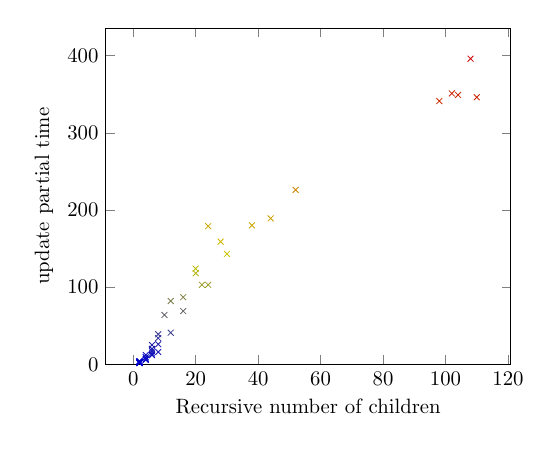
\begin{tikzpicture}[scale=0.75]
\begin{axis}[ymin=0, xlabel={Recursive number of children}, ylabel={update partial time}] \addplot[mark=x, color=blue, scatter, only marks] coordinates {
(2,2) (4,7) (2,2) (8,26) (10,64) (12,82) (2,2) (2,2) (6,17) (2,2) (2,2) (6,20) (8,34) (2,4) (2,3) (6,12) (16,69) (24,103) (38,180) (2,4) (4,12) (44,189) (2,2) (2,2) (4,9) (6,25) (8,39) (2,2) (4,6) (6,12) (16,87) (20,118) (22,103) (24,179) (2,3) (28,159) (30,143) (2,3) (4,9) (6,20) (2,2) (2,2) (2,2) (6,14) (8,16) (12,41) (20,124) (52,226) (98,341) (2,2) (102,351) (104,349) (2,3) (108,396) (110,346) (2,2) (4,6) };
\end{axis}
\end{tikzpicture}
\end{minipage}
